\documentclass[tikz,border=8pt]{standalone}
% Shared look for every TikZ diagram. Load with \input{../../tools/tikz-style.tex}
\usepackage[T1]{fontenc}
\usepackage{lmodern}
\renewcommand{\sfdefault}{lmr}  % diagrams use the same serif as the text
\usetikzlibrary{arrows.meta, positioning, shapes.geometric, calc, fit, backgrounds}
\definecolor{cblue}{HTML}{4C78A8}
\definecolor{corange}{HTML}{F58518}
\definecolor{cgreen}{HTML}{54A24B}
\definecolor{cred}{HTML}{E45756}
\definecolor{cpurple}{HTML}{B279A2}
\definecolor{cgrey}{HTML}{6B6B6B}
\tikzset{
  every picture/.style={font=\sffamily, line width=1.2pt},
  box/.style={draw=#1, fill=#1!12, rounded corners=4pt, align=center, inner sep=7pt, minimum height=1.1cm},
  box/.default=cgrey,
  arrow/.style={-{Stealth[length=3mm]}, draw=cgrey, line width=1.4pt},
  title/.style={font=\sffamily\bfseries\Large},
  note/.style={font=\sffamily\small, text=cgrey, align=center},
}
\AtBeginDocument{\hyphenpenalty=10000 \exhyphenpenalty=10000}

\begin{document}
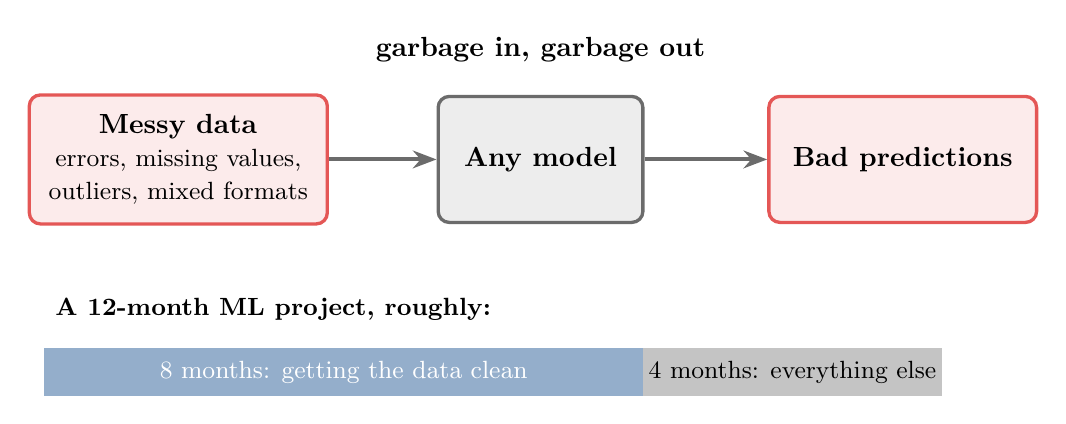
\begin{tikzpicture}
  \node[box=cred, minimum width=3.4cm, minimum height=1.6cm, align=center] (in) at (0,0) {\textbf{Messy data}\\{\small errors, missing values,}\\{\small outliers, mixed formats}};
  \node[box=cgrey, minimum width=2.6cm, minimum height=1.6cm] (m) at (4.6,0) {\textbf{Any model}};
  \node[box=cred, minimum width=3.4cm, minimum height=1.6cm] (out) at (9.2,0) {\textbf{Bad predictions}};
  \draw[arrow] (in) -- (m); \draw[arrow] (m) -- (out);
  \node[font=\bfseries] at (4.6,1.4) {garbage in, garbage out};
  % time spent on a 12-month project
  \node[anchor=west, font=\small\bfseries] at (-1.7,-1.9) {A 12-month ML project, roughly:};
  \fill[cblue!60] (-1.7,-3.0) rectangle ++(8*0.95,0.6);
  \fill[cgrey!40] (-1.7+8*0.95,-3.0) rectangle ++(4*0.95,0.6);
  \node[font=\small, text=white] at (-1.7+4*0.95,-2.7) {8 months: getting the data clean};
  \node[font=\small] at (-1.7+10*0.95,-2.7) {4 months: everything else};
\end{tikzpicture}
\end{document}
